\section{Experiments}
\label{experiments}

%For the following two experiments, the pacemaker model is evaluated against two physiological requirements.
a) \emph{Exploring behavior}: In this experiment, we
%set a minimum delay of 400ms between PVC pulses, and 
tried to falsify the following specification:
``The interval between an activation of the ventricle node to a ventricular pacing (VP) should be longer than 500ms".
This specification is designed to identify closed-loop execution traces in which the pacemaker is pacing the heart too fast. %Note that the pacemaker can not distinguish between a VS caused by a PVC and a VS caused by path conduction.
%Thus we need access to the heart model to test this specification, and this can only happen in a closed-loop setting.

The specification was violated by the execution shown in Fig. \ref{fig:bug8_kept1}.
% This comes from bug8_kept1
\begin{figure}[tb]
\centering
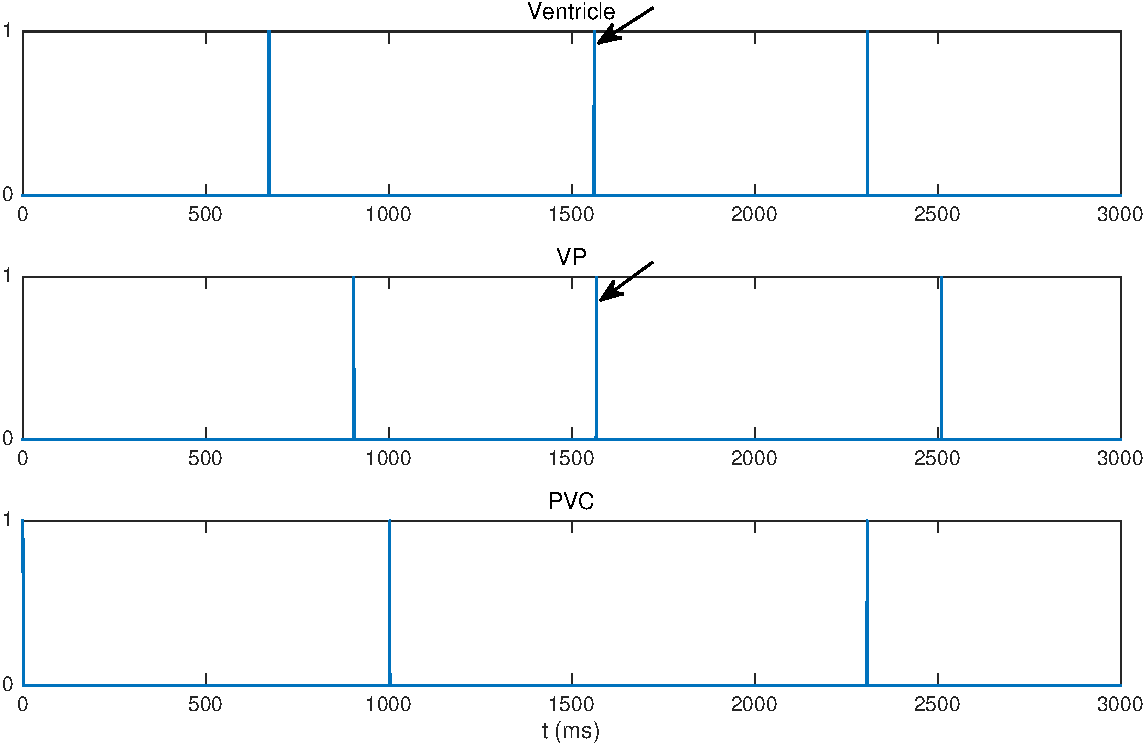
\includegraphics[width=0.7\linewidth]{figures/bug8_kept1}
\caption{A PVC pattern that causes a premature ventricular pacing.}
\label{fig:bug8_kept1}
\end{figure}
Upon investigating the reasons for this violation, it was concluded that one of the noise filters, the post-atrial ventricular blocking (PAVB) designed to avoid crosstalk between channels, caused the problem.  
A PVC happened shortly after an atrial sense (AS) which fell into the PAVB period and was ignored. 
Due to its limited sensing capability the pacemaker cannot distinguish noise from a valid input which happened at a rare time.
Thus, the designer and physician must decide whether this is an acceptable case, or the pacemaker needs to be adjusted (if at all possible) to prevent this from happening (while maintaining the VSP safety feature).

b) \emph{Finding harmful heart behavior}: In this experiment, we tested the closed loop to see if the pacemaker could lead the heart into a harmful condition known as Endless Loop Tachycardia (ELT).
%
The heart has one intrinsic conduction pathway from atria to ventricles, namely from the SA node to the ventricles via the AV node and His bundle.
The AVI period of the DDD pacemaker introduces another, virtual, pathway between the atrial lead and the ventricular lead.
See Fig.~\ref{fig:nodesandPM}.
%If a PVC happens shortly after a normal A-to-V conduction, the signal would go around the closed circuit formed by the heart and the pacemaker, inhibiting intrinsic heart signals and causing the heart to beat at a fixed high rate.
In an ELT, first, a PVC triggers V-A conduction along the intrinsic pathway, 
which in turn triggers an AS. 
The pacemaker will then pace the ventricle (issue a VP) after TAVI ms according to its A-V synchrony function. 
This VP then triggers another V-A conduction, and so on.
The conduction loop is then formed and the VP-AS pattern will persist if no actions are taken,
and the heart rate is kept as high as the upper rate limit of the pacemaker.% since the cycle length of the conduction loop is very short. 
As shown in Fig.\ref{fig:ambiguity}, the pacemaker's limited sensing capabilities can not distinguish between a PVC-induced VS and an intrinsic VS.
ELT is a harmful condition since a fast fixed heart rate that will cause inefficient pumping of blood.
Thus even though the pacemaker is correct according to its specification, it can still lead the heart into ELT if a PVC interferes with its operation as described.
%
\begin{figure}[t]
\centering
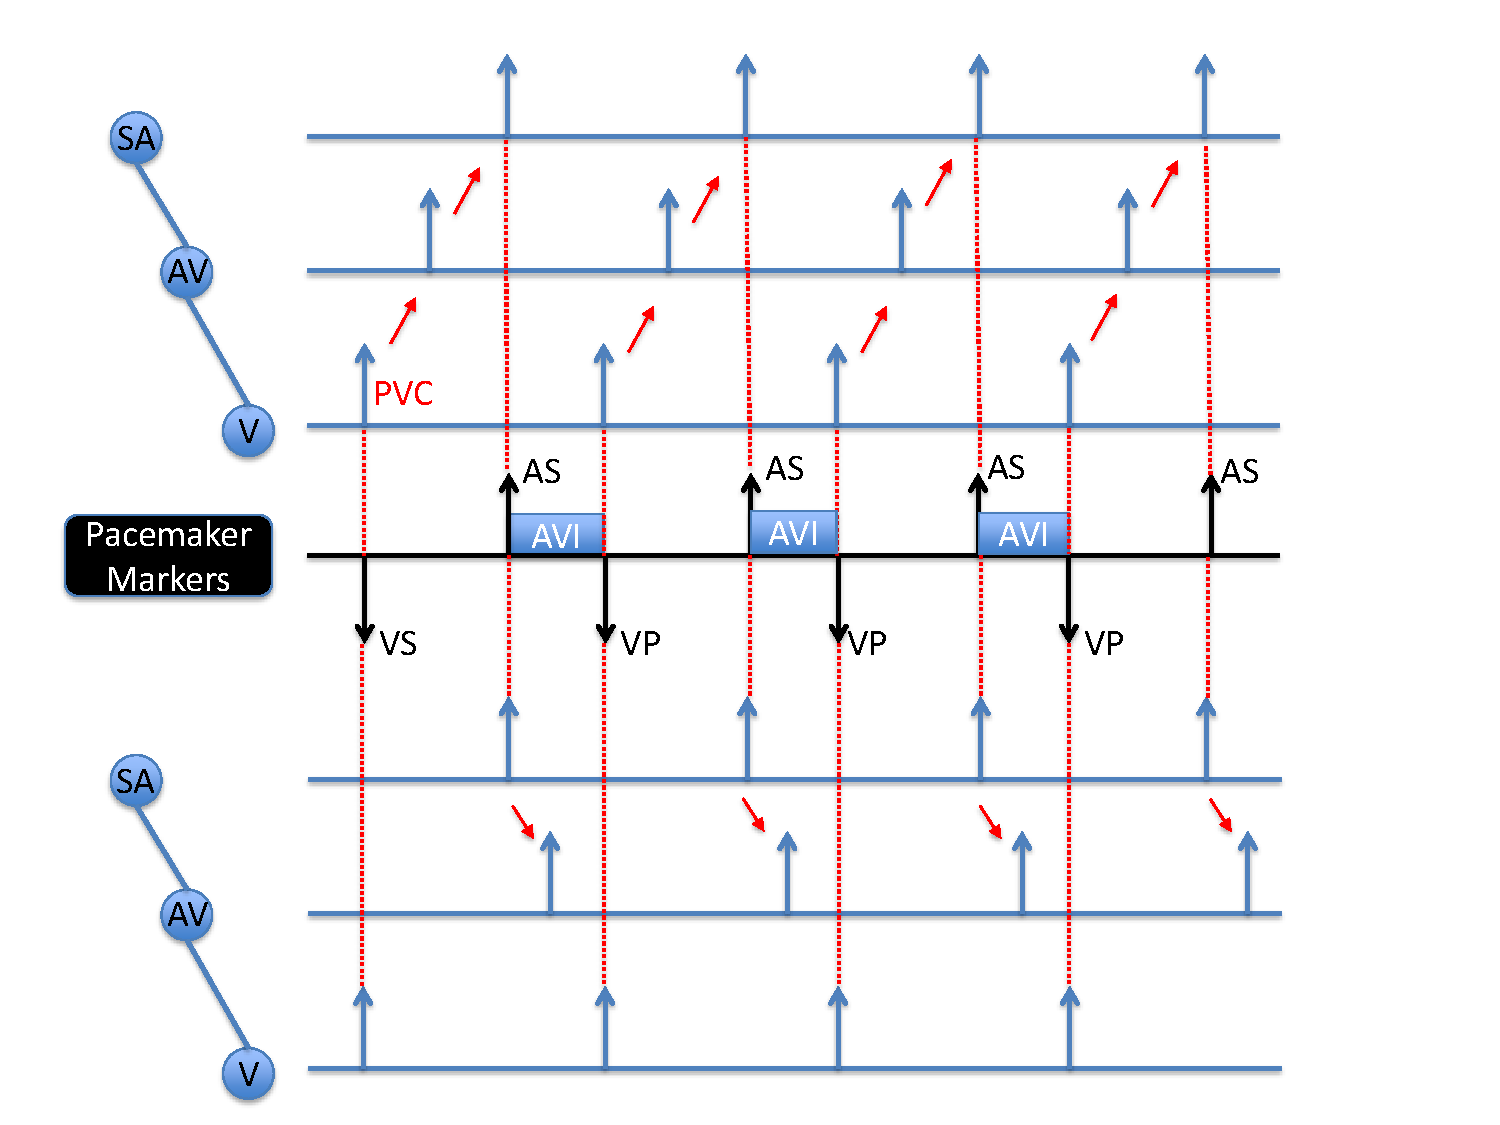
\includegraphics[scale=0.3]{figures/ambiguity}
\caption{An ELT sequence (above the Markers line) and an intrinsic conduction (below it) cause the same sensed events in the pacemaker.}
\label{fig:ambiguity}
\vspace{-0.7cm}
\end{figure}
S-Taliro was given the ELT specification, and a PVC constraint of at most 2 PVCs in a 10,000ms interval. 
The total test duration was $T= 10,000$ms.
S-Taliro found a PVC pattern, shown in Fig.~\ref{fig:bug13_kept1}, that caused ELT.
% This is bug13_kept1
\begin{figure}[t]
\centering
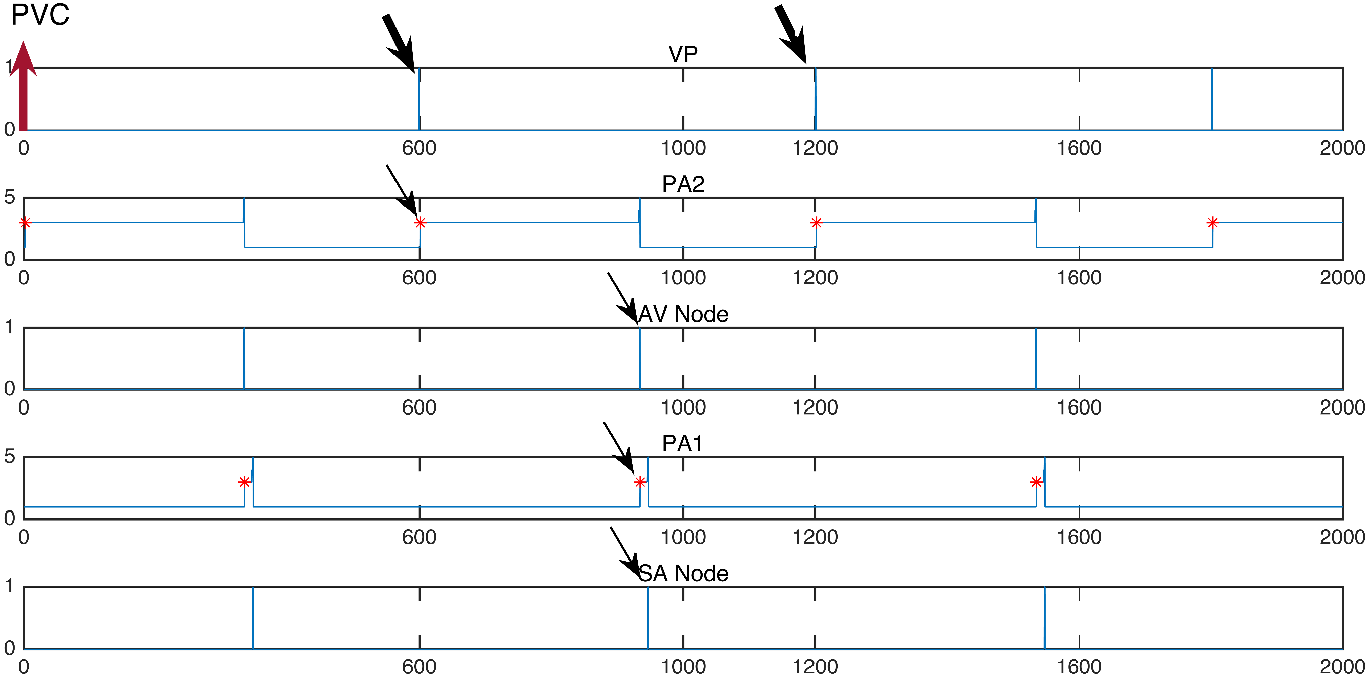
\includegraphics[height=0.2\textheight,width=1\columnwidth]{figures/markedELT.pdf}
\caption{ELT. The vertical red arrow indicates the initial PVC, thick arrows indicate the beginning of each ELT cycle, and thin arrows indicate the events involved in the ELT diagnosis.}
\label{fig:bug13_kept1}
\end{figure}


